\documentclass[../thesis.tex]{subfiles}

\begin{document}

\chapter{Decision Support Tool for Multi-Hospital Planning of Frail and Elderly Resource Capacities}\label{chp:tool}

\section{Introduction}
This chapter will provide a tutorial guide on how to use the two tools discussed within Chapters \ref{chp:Experimental Analysis} and \ref{chp:Linking}. These tools are adaptable so can be applied to other healthboards and scenarios or other patient groupings. Section \ref{sec:excelimp} will discuss the Microsoft Excel OpenSolver Tool which is specific to ABUHB. Section \ref{sec:pythonimpl} discusses the Python PuLP implementation of the model, which can be generalised to any healthboard situation.



%of the two tools used within Chapter \ref{chp:Experimental Analysis}.
want to be reproducible for future
applicable to other healthboards, scenarios
other patient types

The remainder of the chapter is as follows: Section \ref{sec:excelimp} will provide an overview of the Microsoft Excel OpenSolver tool and Section \ref{sec:pythonimpl} provides an overview of the Python PuLP model.


\section{Excel Implementation}\label{sec:excelimp}
Microsoft Excel is a widely-used tool for data analysis and management, and OpenSolver is a powerful optimisation engine that can be used to solve complex problems within Excel. In this guide, we will provide step-by-step instructions on how to run the OpenSolver model, from setting up your data and formulating your problem to running the optimisation and analyzing the results

The OpenSolver model without the ABUHB data has been provided on Github \cite{}\hl{Add in ref} to allow readers and users to enter their own data and hospital specialties. The tool consists of of multiple sheets for details such as . Each type of parameters has its own individual sheet, and is clearly names to ensure the planners can easily access data. Due to the limitations of the software, all decision variables in the optimisation model must be on the same sheet, and thus to prevent important these from being altered are stored in protected sheets. For visualisation purposes the decision variables are automatically transferred into the model sheets after the experiment has run.

\subsection*{Data}
Figure \ref{fig:exdata} displays the data which is used by the model. This is stored within the `Data' tab and allows users to enter and change the parameters to suit their model. The user is required to enter the specialty that a patient is admitted to and the hospital where they are admitted. The `Short LOS' determines the number of nights spent in hospital, whilst the `LOS\_hours' determines the continuous time spent in hospital. Additionally, the date tab can be added if the user wishes to split their model by year, season, month or days of the week. Finally there is the NHS Patient Identifier which is unique to the patient.

\begin{figure}[h!]
    \centering
    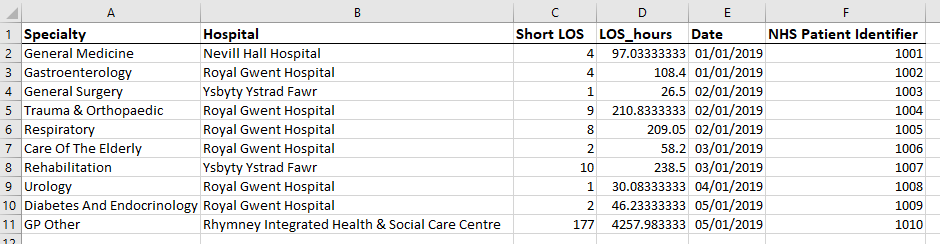
\includegraphics[width=\textwidth]{Chapters/Chapter7/Figures/Data.png}
    \caption{OpenSolver Tool - Data Requirements}
    \label{fig:exdata}
\end{figure}

%The data for the models is stored within the `Data' tab, where users can input their specific data into one of the six columns .


\subsection*{Demand}
The demand for each speciality is automatically generated from the data inputted by the user, and is stored within the `Demands' tab within the Excel spreadsheet. The average demand is calculated by determining if a specialty and hospital combination is present and if so calculating the total for each combination. Similarly, if patients do fall within these combinations then the average LOS, using `LOS\_hours', is calculated for each specialty and hospital. These values are then multiplied together and subsequently divided by 24, as the LOS is given in hours, and then by the total number of days in the data, to give a daily demand. This means if a user wants to determine a monthly demand, the `Number of Days in Data' can be changed to the number of months within the data. This is then stored as a table shown in Figure \ref{fig:exdemand}.
\begin{figure}[h!]
    \centering
    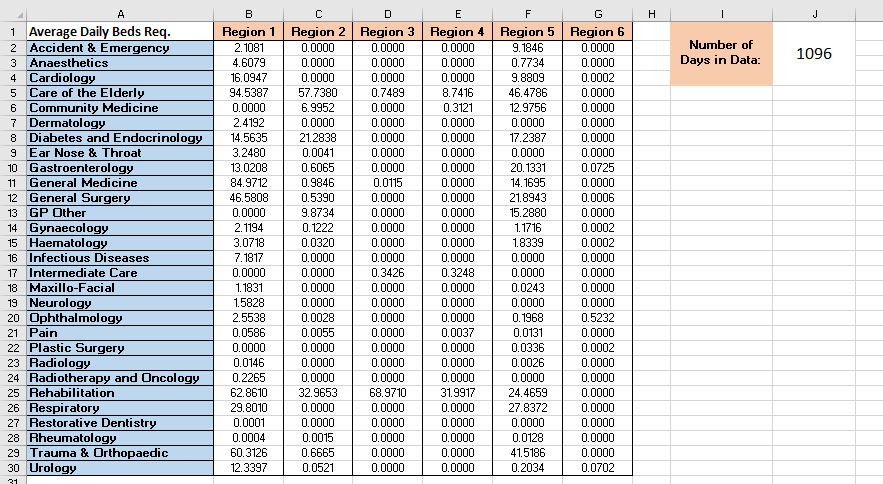
\includegraphics[scale=0.8]{Chapters/Chapter7/Figures/Demands.png}
    \caption{OpenSolver Tool - Demand}
    \label{fig:exdemand}
\end{figure}

\subsection*{Possible Hospital Locations}
The tab entitled `Hospital-Specialty' contains data regarding whether a hospital is able to open a specialty within a specific hospital. In order to restrict the number of beds that can be deployed in hospital location, the total bed capacity for the 1$^{st}$ and 2$^{nd}$ stages of the model can be seen within Figure \ref{fig:exlocations}. As some hospitals may not be able to open full capacity to one speciality, due to resource or space limitations, the user is able to reduce these values whilst still being able to open up to the full capacity across other specialties. If a value of zero is present, this means the hospital is unable to open that specialty.
\begin{figure}[h!]
    \centering
    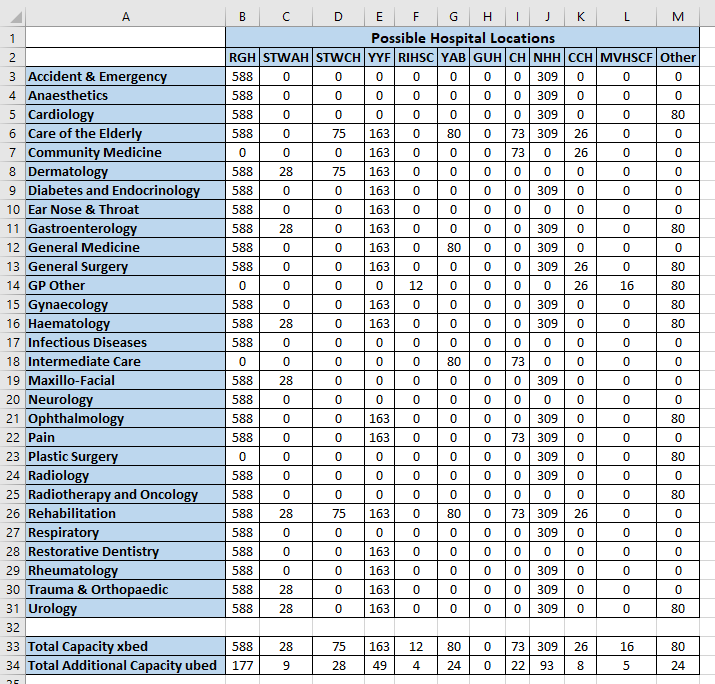
\includegraphics{Chapters/Chapter7/Figures/Hospital-Spec.png}
    \caption{OpenSolver Tool - Possible Hospital Locations}
    \label{fig:exlocations}
\end{figure}

\subsection*{Hospital Costs}
Within the `Hospital Costs' tab in the spreadsheet, the user is able to enter the average daily cost for each specialty. Similar to demands, if the user wants to work in a different time frame; monthly, seasonally, or yearly, the cost figures can also be adjusted. Figure \ref{fig:excostings} displays the 1$^{st}$ stage hospital costs, with an identical matrix grid being found below in the spreadsheet. 
\begin{figure}[h!]
    \centering
    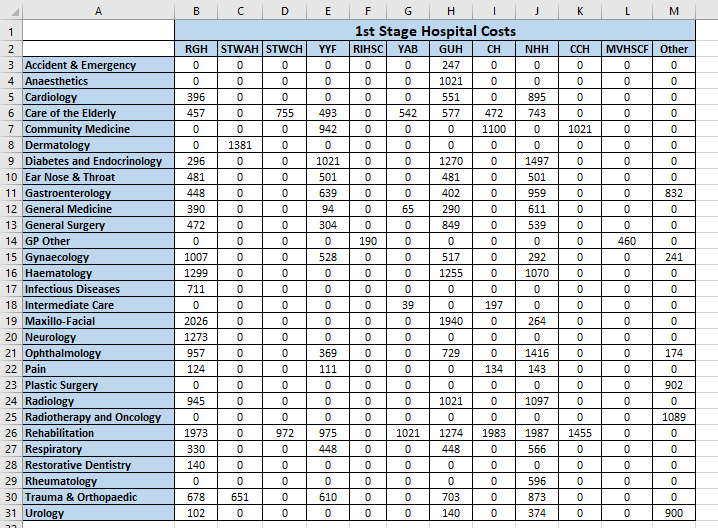
\includegraphics{Chapters/Chapter7/Figures/Costings.png}
    \caption{OpenSolver Tool - Hospital Costings}
    \label{fig:excostings}
\end{figure}

\subsection*{Staffing}
The `Staffing' tab in the Excel worksheet contains all the information required for the staffing requirement. Firstly the ratios of staff to patients can be altered depending on the band level and the specialty (Figure \ref{fig:exstaff}). The hourly and daily cost per staff can also be changed. This flexibility allows pay rises to be included and flexibility in costings across other countries. Similarly, the cost of NHS bank and agency staff is also included. Finally, the maximum number of staff that can be deployed both in the first and second stages are detailed. One limitation of the excel model is higher levels of staff cannot perform the job of the lower band staff members. This is due to the non-linearity of the constraint which the COIN-OR CBC (Linear solver) cannot handle.

\begin{figure}[h!]
    \centering
    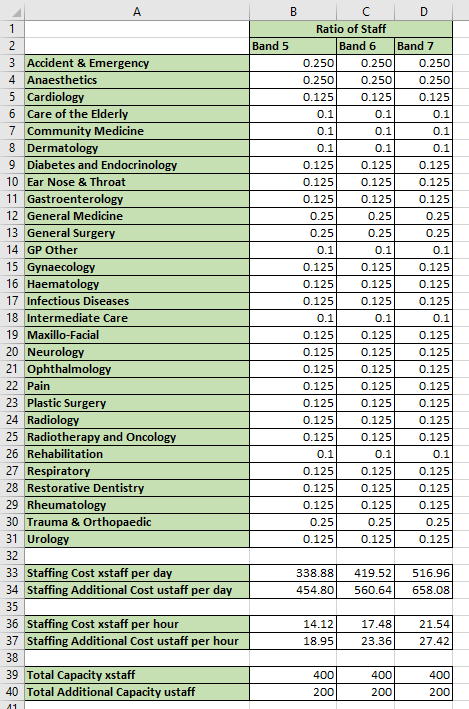
\includegraphics{Chapters/Chapter7/Figures/Staff.png}
    \caption{OpenSolver Tool - Staffing}
    \label{fig:exstaff}
\end{figure}

\subsection{Deterministic Model}
The deterministic model is stored within the `Deterministic' tab, here the optimisation model can be run and the results analysed. With the OpenSolver add-in installed, the model can be easily accessed through the Data ribbon and then selecting the Model on the OpenSolver toolbar. This brings up Figure \ref{fig:exdmos}, which depicts the objective function cell, the type of problem (maximisation or minimisation), the decision variables, the models constraints and the type of solver engine. Using the options button; the maximum solution time, branch and bound tolerance and the maximum number of iterations can also be changed. To solve the model, the `Solve' button can be selected on the OpenSolver \hl{ribbon}.

\begin{figure}[h!]
    \centering
    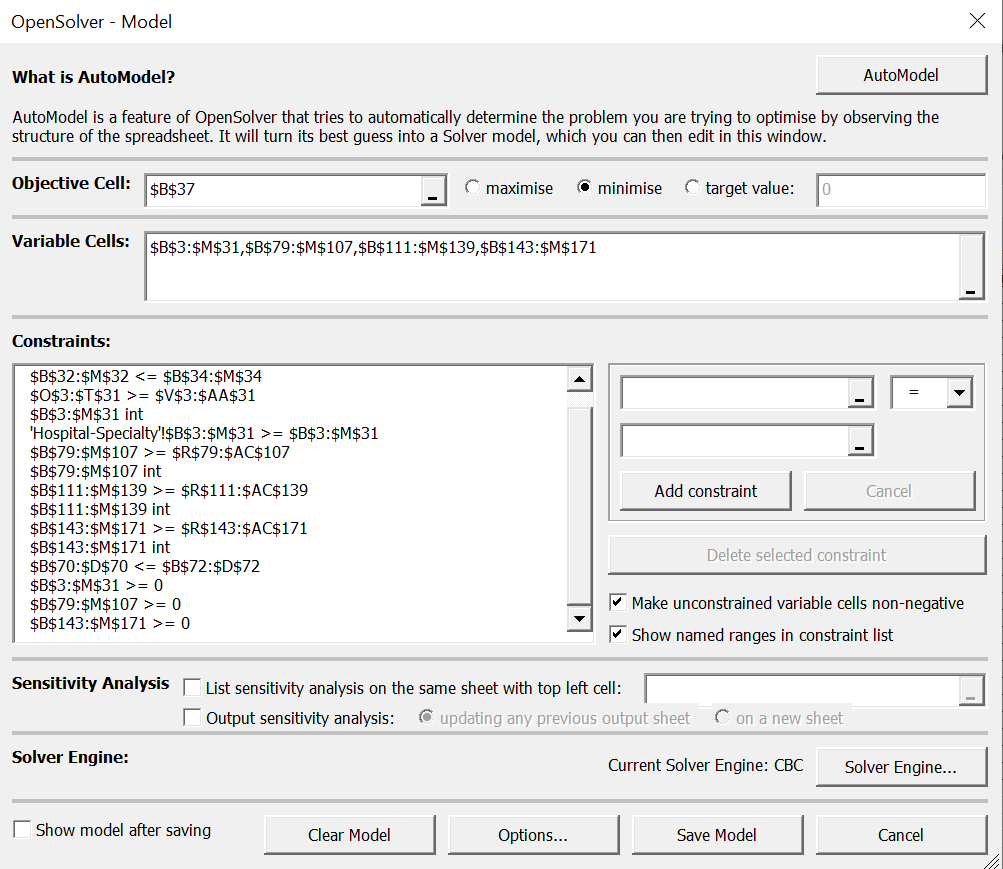
\includegraphics[scale=0.5]{Chapters/Chapter7/Figures/DeterministicOS.png}
    \caption{OpenSolver Tool - Deterministic Model}
    \label{fig:exdmos}
\end{figure}
Once executed, the total cost of the model is shown within the sheet, along with the total number of beds and staff to be deployed (Figure \ref{fig:exdm1}). The model shows where each of these beds should be deployed across the specialties and hospitals 

\begin{landscape}
\begin{figure}[h!]
    \centering
    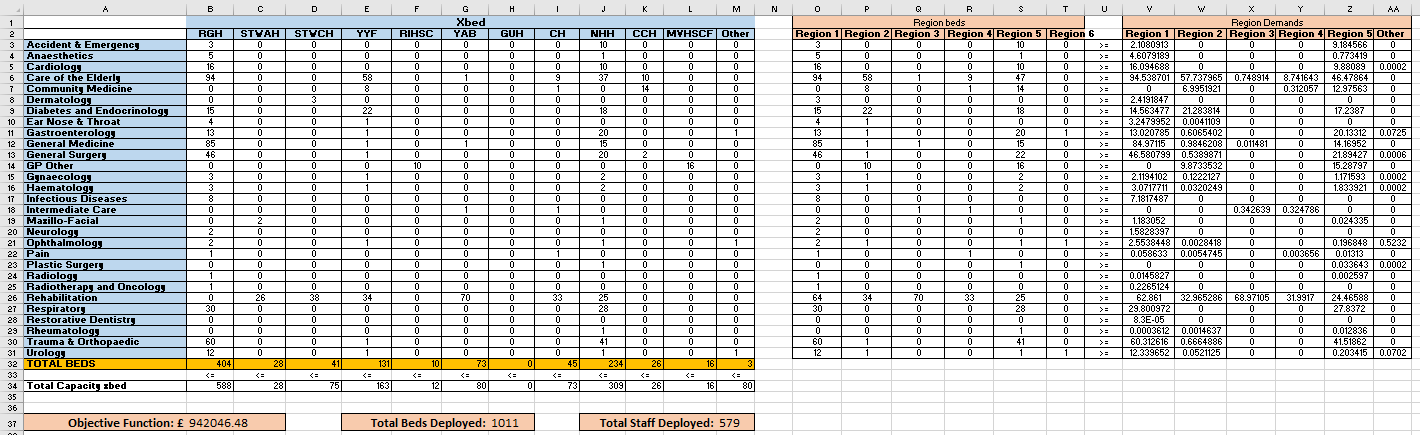
\includegraphics{Chapters/Chapter7/Figures/Deterministic1.png}
    \caption{OpenSolver Tool - Deterministic Model 1}
    \label{fig:exdm1}
\end{figure}
\end{landscape}
\begin{figure}
    \centering
    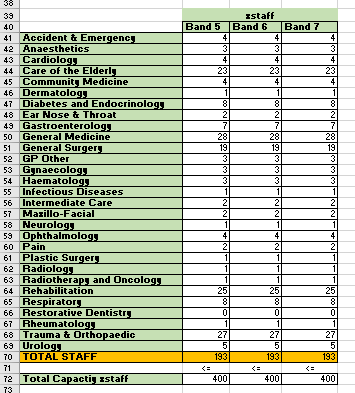
\includegraphics{Chapters/Chapter7/Figures/Deterministic2.png}
    \caption{OpenSolver Tool - Deterministic Model 2}
    \label{fig:exdm2}
\end{figure}



% \subsection{Parameters}
% There are \hl{Y} Excel sheets containing the









% \subsection{}
% \subsection{Constraints or Open Solver Equations?}
% \subsubsection{Deterministic}
% The deterministic model contains \hl{X - i think 16?} constraints to ensure

% \begin{itemize}
%     \item minimise
%     \item decision variables
%     \item Solver type
% \end{itemize}
% \subsubsection{Two-Stage Stochastic}
% \subsubsection{Combination}

% \subsection{Result Output and Interpretation}

\section{Python Implementation}\label{sec:pythonimpl}


\end{document}
